%This section should be where you establish the effectiveness of the two denoising methods, including their processing time, by using existing (conventional) feature detectors such as FAST and HARRIS, and a conventional tracking algorithm such as Lucas-Kanade. 
%You should also include your own proposed method in the evaluation.
%
%Also, you should look at the effect of different methods of scaling the 14-bit data to 8-bit format. The advantage of 8-bit format is that it requires less processing time, and also allows more modularity with existing functions and libraries. Furthermore, there should generally be very little (if any) information lost in this conversion, and when information is lost, it means it is a high SNR image and so the loss of the information is not a problem (there is still sufficient information left over).



%We propose a novel image denoising strategy based on an enhanced sparse representation in transform domain. The enhancement of the sparsity is achieved by grouping similar 2D image fragments (e.g., blocks) into 3D data arrays which we call "groups." Collaborative Altering is a special procedure developed to deal with these 3D groups. We realize it using the three successive steps: 3D transformation of a group, shrinkage of the transform spectrum, and inverse 3D transformation. 
%The result is a 3D estimate that consists of the jointly filtered grouped image blocks. By attenuating the noise, the collaborative filtering reveals even the finest details shared by grouped blocks and, at the same time, it preserves the essential unique features of each individual block. The filtered blocks are then returned to their original positions. Because these blocks are overlapping, for each pixel, we obtain many different estimates which need to be combined. Aggregation is a particular averaging procedure which is exploited to take advantage of this redundancy. A significant improvement is obtained by a specially developed collaborative Wiener filtering

In this section, authors would like to establish the effectiveness of the two proposed denoising methods, namely Non-local algorithm \cite{Buades} and Transform-domain collaborative filtering \cite{dabov2007image}. In short, first method analyzes noise for  local smoothing filters followed by computing nonlocal means whilst second approach groups 2D image fragments into 3D data arrays to unveil the finest details based on aggregation and collaborative Wiener filtering.  

Compare to Transform-domain collaborative filtering in terms of processing time, Non-local means is about 5 time faster. However, in terms of output quality, Transform-domain collaborative filtering is incomparable and still state-of-the-art method for denoising target. As a result, we propose to employ first denoising technique in case of low noise level. Otherwise, second approach is used to ameliorate further-processing steps. To classify whether an image is noisy or not, we profound applying an estimation of noise level based on Bayesian MAP inference \cite{liu2006noise} and analogizing to a predefined threshold of 5 (for 0-255 grayscale) (need to find this threshold!?).

To evaluate the effectiveness of two proposed denoising methods, two thermal images with different level of SNR are introduced. Next, feature detectors, namely FAST \cite{rosten2006machine} and HARRIS \cite{harris1988combined}, are deployed in noisy and denoised frames for collation. The  minimum accepted quality of corners and minimum intensity parameters \footnote{http://www.mathworks.com/help/vision/ref/detectfastfeatures.html}, are set at 0.005 in both methods and 0.05 in FAST, respectively.  The results are shown in Fig. \ref{fig:imgprocessing}.

\begin{figure}
\centering
	\begin{subfigure}{0.49\columnwidth}
    \centering
    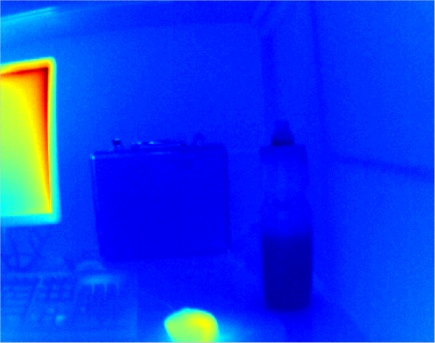
\includegraphics[width=1.00\textwidth]{media/V_C_highsnr.jpg}
	    \caption{}
		\label{fig:imgprocessing_1}
  \end{subfigure}
	\begin{subfigure}{0.49\columnwidth}
    \centering
    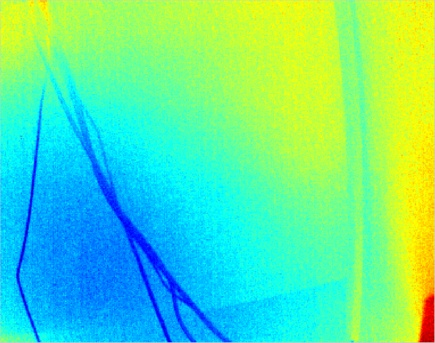
\includegraphics[width=1.00\textwidth]{media/V_C_lowsnr.jpg}
		\caption{}
		\label{fig:imgprocessing_2}
  \end{subfigure} \vspace{10pt} \\ 
	\begin{subfigure}{0.49\columnwidth}
    \centering
    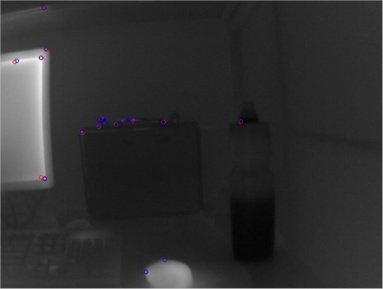
\includegraphics[width=1.00\textwidth]{media/V_C_highsnrcornersori.jpg}
    	\caption{}
		\label{fig:imgprocessing_3}
  \end{subfigure}
	\begin{subfigure}{0.49\columnwidth}
    \centering
    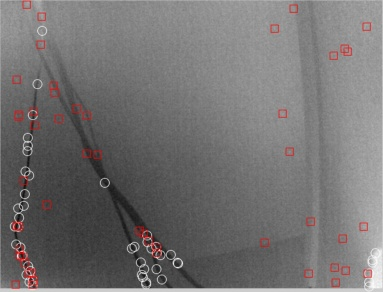
\includegraphics[width=1.00\textwidth]{media/V_C_lowsnrcornersori.jpg}
		\caption{}
		\label{fig:imgprocessing_4}
  \end{subfigure} \vspace{10pt} \\ 
	\begin{subfigure}{0.49\columnwidth}
    \centering
    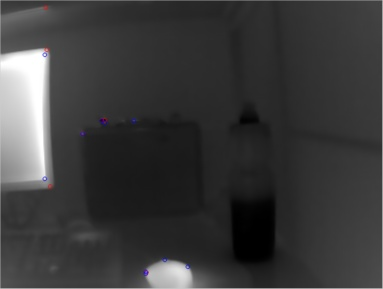
\includegraphics[width=1.00\textwidth]{media/V_C_highsnrcornersnonlocal.jpg}
    	\caption{}
		\label{fig:imgprocessing_5}
  \end{subfigure}
	\begin{subfigure}{0.49\columnwidth}
    \centering
    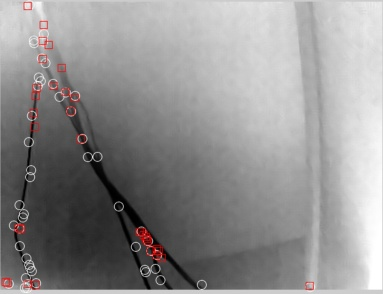
\includegraphics[width=1.00\textwidth]{media/V_C_lowsnrcornersnonlocal.jpg}
		\caption{}
		\label{fig:imgprocessing_6}
  \end{subfigure} \vspace{10pt} \\ 
	\begin{subfigure}{0.49\columnwidth}
    \centering
    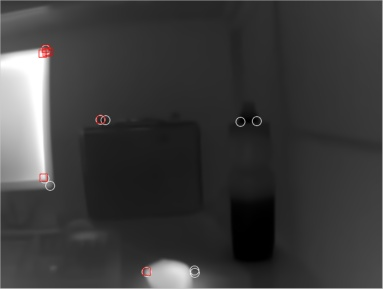
\includegraphics[width=1.00\textwidth]{media/V_C_highsnrcornerstrans.jpg}
    	\caption{}
		\label{fig:imgprocessing_7}
  \end{subfigure}
	\begin{subfigure}{0.49\columnwidth}
    \centering
    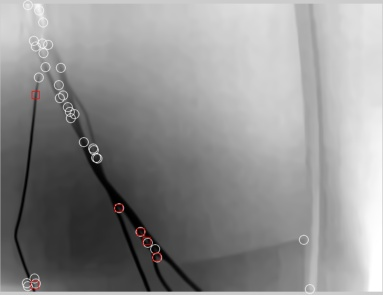
\includegraphics[width=1.00\textwidth]{media/V_C_lowsnrcornerstrans.jpg}
		\caption{}
		\label{fig:imgprocessing_8}
  \end{subfigure}
\caption{Image processing evaluation: (a,b) original indoor high and low SNR frames, (c,d) gray-scale frames, (e,f) non-local means denoised frames, (g,h)  transform-domain collaborative filtering denoised frames, white circles and red rectangular denote feature points by Harris and FAST methods, respectively}
\label{fig:imgprocessing}
\end{figure}


%MinQuality 0.005 - both
%MinContrast 0.05 - Fast
%corners1 = detectHarrisFeatures(grayImage,'MinQuality',0.005);
%corners2=detectFASTFeatures(grayImage,'MinQuality',0.005,'MinContrast',0.05);
%A=corners1.selectStrongest(50).Location;
%B=corners2.selectStrongest(50).Location;
%figure;imshow(grayImage);axis off;hold on
%scatter(A(:,1),A(:,2),50,'w');
%scatter(B(:,1),B(:,2),50,'r','s');
%export_fig V_C_lowsnrcornersori.jpg


%In high SNR thermal images, such as Fig. \ref{fig:imgprocessing_1}, both denoising methods output 


Fig. \ref{fig:imgprocessing} shows that 

The table shows that the figures for imprisonment in the five countries mentioned indicate no overall pattern of increase or decrease. In fact there is considerable fluctuation from country to country.